



\section{Section 2: Wireless networks}

In this section, communication networks are presented, with special attention to wireless technologies. An historic overview is presented 



1.	Network technologies – historic overview

2.	Current technologies and standards:

3.	Emerging technologies and standards

4.	Network Simulators and Network Emulators






\subsection{Network technologies – historic overview}


\subsection{Current Wireless technologies and standards}

The following sections will cover the wireless communications in smart metering systems, starting with the low-rate and low-power communications applied around the smart meters and ending with the high-rate communications (and consequently higher costs and power than low rate communications). With the increasing on demand for higher bandwidth, broadband technologies such as mobile WiMAX, IEEE 802.16e and broadband PLC are expected to be considered and used in newer installations, \cite{Mohassel2014}.


%As the demand for bandwidth increases, broadband technologies such as IEEE 802.16e, mobile WiMAX and broadband PLC are going to play a key role in newer installations, \cite{Mohassel2014}.

\subsubsection{IEEE 802.11 (Wireless LAN (WLAN) or Wi-Fi)}

IEEE 802.11 is the standard for the information exchange between systems and for the telecommunications. The coverage area of this technology is on local and metropolitan area networks (LANs and MANs). The specific requirements are on the Medium Access Control and on Physical Layer. The most popular versions of this standard is the IEEE 802.11b and IEEE 802.11g, that differs in the modulation technique (Direct Sequence Spread Spectrum (DSSS) technique versus Orthogonal Frequency Division Multiplexing (OFDM) modulation technique). The data rates are, respectively, 11 Mbps and 54 Mbps, \cite{Usman2013, ieee2012}.



\subsubsection{IEEE 802.15.4 (ZigBee)}

The standard IEEE 802.15.4 imposes conditions in the physical layer and media access control focusing on low-rate (up to 300 kHz) wireless personal area networks. Developed by the Zigbee Alliance and covering the specifications of the IEEE 802.15.4 on the physical layer and the medium access control, Zigbee is a commonly used for low power wireless communication technology. It operates on the ISM bands of 868 MHz, 915 MHz and 2.4 GHz adopting direct sequence spread spectrum (DSSS), \cite{Usman2013}.

%IEEE 802.15.4 is a standard that specifies the physical layer and media access control for low-rate (up to 300kHz) wireless personal area networks. ZigBee is a popular, low power wireless communication technology developed by the ZigBee Alliance based on the Physical Layer and Media Access Control Layer of the IEEE 802.15.4 standard.
%It operates on the ISM bands of 868 MHz, 915 MHz and 2.4 GHz adopting direct sequence spread spectrum (DSSS), \cite{Usman2013}.


\subsubsection{DASH7}

On the low-rate field of research, an alternative to Zigbee is the DASH7. Using the ISO/IEC 18000-7 standard to support this wireless sensor network technology, DASH7 is developed to reach active Radio Frequency Identification Devices (RFIDs) and operates at 433MHz band. The advantage is the typical range of 250m (could achieve 5 km) and has a typical and maximum data rates of 28 kbps and 200 kbps, being in this specifically designed for Smart Grid and for applications in Smart Energy.


\subsubsection{6LoWPAN}

IEEE 802.15.3: IEEE 802.15.3 [46] is a physical and MAC
layer standard for high data rate WPAN. It is designed to
support real-time multi-media streaming of video and music.
IEEE 802.15.3 operates on a 2.4 GHz radio and has data
rates starting from 11 Mbps to 55 Mbps

\subsubsection{Wibree}

Wibree [47] is a wireless communication technology
designed for low power consumption, short-range
communication, and low cost devices. Wibree allows the
communication between small battery-powered devices
and Bluetooth devices. Small battery powered devices include
watches, wireless keyboard, and sports sensors
which connect to host devices such as personal computer
or cellular phones. Wibree operates on 2.4 GHz and has a
data rate of 1 Mbps. The linking distance between the devices
is 5–10 m. Wibree is designed to work with Bluetooth.
Bluetooth with Wibree makes the devices smaller
and more energy-efficient. Bluetooth–Wibree utilizes the existing Bluetooth RF and enables ultra-low power consumption.
Wibree was released publicly in October 2006.


\subsubsection{Industrial Wireless Communications: WirelessHART and ISA100.11a}

Launched by HART Communication Foundation in September of 2007, WirelessHART is an open wireless communication standard designated specifically for the process measurement and control applications, \cite{Song2008}. This standard is specifically designed to comply with industrial requirements, such as stricter timing requirement, higher security concern, immunity to harsher interferences and obstacles and enough scalability to be used in large process control systems.

Similarly, ISA100.11a aims to provide secure and reliable wireless communication for noncritical monitoring and control applications, \cite{Petersen2011}.





\subsubsection{IEEE 802.16 (WiMAX)}

On the field of the broadband wireless communication there is the Worldwide Interoperability for Microwave Access (WiMAX) under the IEEE 802.16 standard. It is specifically developed aiming the point-to-multipoint communications being applied in fixed and mobile applications and it has data rates up to 70 Mbps over a distance of 50 km. Framed into the smart grid systems, this communication technology is considered as a solution for high data rate communication link to be applied at the backbone of the utilities, \cite{Usman2013}.


\subsubsection{Broadband communications: GSM/GPRS and LTE/LTE-Advanced}

Operating at 900 MHz and 1800 MHz, the Global System for Mobile communications (GSM) is the most used cellular network all over the world. The modulation technique is the Gaussian Minimum Shift Keying (GMSK) and it achieves transfer rates up to 270 kbps. Its architecture consists of four components: the Operation Support Substation, the Network Switching Substation, the Base Station Subsystem and the Mobile handset. Due to its level of development around the world being present in remote locations, this advantage makes this  an interesting technology to be applied in Smart Grid applications, \cite{Usman2013}.

Long Term Evolution (LTE) is a recent standard for wireless technology that allows high data rates with high capacity and low latency and with a good Quality of Service (QoS). The improved version of this technology, the LTE-Advanced, admit higher capacity with expanded peak data rate of 1 Gbps for the downlink and 500 Mbps for the uplink, obtained on the increase of the spectral efficiency, higher  number of active subscribers connected at the same time, and better performance at cell edges, \cite{Mohassel2014}. This technology, for the Smart Metering environment where the high bandwidth and good QoS are mandatory at some communication points.




\subsection{Emerging Technologies and Research Trends}

ver livro khan

\subsection{Network Simulators and Network Emulators}

Several techniques have been introduced for performance evaluation of protocols and algorithms in USN, including analytical modeling,
simulation, emulation, testbed, and real-world experimentation (Imran
et al., 2010). Analytical models are a set of equations that represent the
performance of a system. Although analytical models simplify the
modeling procedure, they cannot accurately represent the inherent
complexity of sensor networks (Krop, 2007). Simulation has been cited
as the most frequent and effective method for designing and developing
network protocols and algorithms (Imran et al., 2010). By using
simulators various scenarios of the real environment can be modeled.
Also, they provide the possibility of testing and debugging protocols at
any stage of design. Emulation, as a hybrid method, is a combination of
hardware and software components accompanying simulation possibilities for network modeling (Kiess and Mauve, 2007). Emulators use

\begin{figure}[h!]
	\centering
	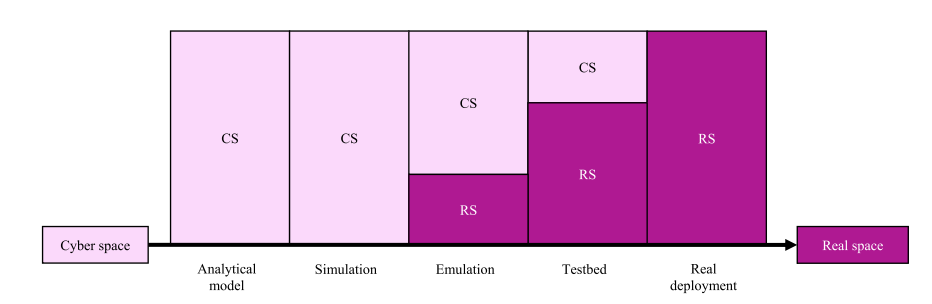
\includegraphics[width=0.65\textwidth,keepaspectratio]{figures/simul_VS_emul}
	\caption{FIGURE TO BE RENAMED.}
	
\end{figure}

An extensive review on simulation tools, made by \cite{nayyar2015}, is presented as following:

\begin{description}
	\setlength\itemsep{0.5em}
	%%1
	\item [NS-2 (network simulator-2)] 
	Object orientated discrete event simulator tool, based on two languages (C++ and OTcl). 
	
	%%2
	\item [NS-3 (network simulator-3)] 
	Written in pure C++, this simulator has been extensively explored in the literature with various modules like 802.15.4, 6LoWPAN and RPL available.
	
	%%3
	\item [OMNET++] 
	This simulator is based in C++ in the basic modules and uses Network DEscription (.NED) scripts to connect and assemble the simulation basic modules.

	%%4
	\item [J-Sim] 
	JavaSim Simulator has been developed in Java and it has several advantages to carry out large scale WSN simulations.

	%%5
	\item [Mannasim] 
	Is based on NS-2 to perform WSN simulations.

	%%6
	\item [SensorSim] 
	Similarly to Mannasim, this is a framework for WSN based on NS-2 simulator. However it is not available, currently, to the public. 

	%%7
	\item [NRL Sensorsim] 
	This extension to NS-2 simulator is focused on WSN, similarly to SensorSim and Mannasim frameworks. Currently, it is no longer in development and does not have support.

	%%8
	\item [NCTUns 6.0] 
	On the field of network emulators, this software has the main advantage of using the real world Linux TCP/IP stack and implements almost every IEEE network standards. Last release was on 2010.

	%%9
	\item [SSFNet] 
	Java simulator designed especially for WSN's. Last release in 2004.

	%%10
	\item [GloMoSim] 
	Non-commercial simulator (the commercial version is \textit{"QualNet"}) designed for wireless and wired network systems.

	%%11
	\item [QualNet 7.0 + EXata 5] 
	Considered one of the most advanced simulator platform these days, QualNet enables a high fidelity virtual model of network, with an advanced GUI. It has a free academic version.

	%%12
	\item [sQualNet Simulator] 
	Is an extension of QualNet for sensor network specific models. 

	%%13
	\item [OPNET Modeler Suite] 
	Is a powerful collection with an interactive GUI to build network scenarios. It has a free academic edition. 

	%%14
	\item [SENSE] 
	Is a powerful sensor network simulator and emulator.

	%%15
	\item [DRMSim] 
	Is a Java-based software that enables large-scale network simulation.

	%%16
	\item [NetSim] 
	Is a simulator designed for protocol modeling, network research and development and defense applications.

	%%17
	\item [UWSim] 
	This simulator is designed for marine robotics research.

	%%18
	\item [Visual Sense] 
	This modeling and simulation software is designed for wireless and WSN applications, as an extension of Ptolemy II.

	%%19
	\item [Viptos] 
	Is an interface/bridge between TinyOS and Ptolemy II.

	%%20
	\item [PTOLEMY II] 
	Is an open source simulation software, based on Java and with actor-oriented design (where actors are software components, have a concurrent execution and communicate via interconnected ports)
	
	%%21
	\item [SENS] 
	This specific framework for WSN's simulator and emulator that uses a simplified sensor model.
	
	%%22
	\item [SHAWN]	
	Is a customizable sensor network simulator focused on the simulation of the effect caused by a phenomenon (not the phenomenon itself) with scalability and support for extremely large networks. According to SHAWN development repository, last contribution was on 2013.
		
	%%23
	\item [SIDnet-SWANS]
	This Java-based simulator was made to provide a simulation and proof-of-concept platform for application of WSN's.
	Latest version was released in 2011.
	
	%%24
	\item [WSim/Worldsens Simulater/WSNet Simulator]
	This simulator states for being an event-driven simulator for large scale wireless networks. Latest version was released in 2009.

	%%25
	\item [WSN Localization Simulator]
	This is a WSN location simulator stating for being easy, scalable and extendable to many/different localization schemes. It was released in 2013.
	
	%%26
	\item [NetTopo Simulator]
	This framework is an open source simulator designed in Java. Its main objective is to analyze various algorithms in WSN's. 
	
	%%27
	\item [SIDH]
	Is a Java-based simulator focused on the simulation of thousand of sensor nodes.
	
	%%28
	\item [PROWLER]
	The Probabilistic Wireless Sensor Network Simulator is a framework that runs under Matlab and is focused to TinyOS applications.
	
	%%29
	\item [Matlab/Simulink]
	With extensive usage by the research community, Matlab and Simulink software provides resourceful toolboxes for simulation of communication networks, being possible to build a complete WSN model system.
	
	%%30
	\item [PiccSIM]
	This simulation platform uses Matlab/Simuling and NS-2 for networked control systems (in particular wireless)
	
	%%31
	\item [LabVIEW]
	Various toolboxes to simulate WSN's are available with LabVIEW.
	
\end{description}






